\section{Methods for monocular reconstruction of articulated subjects}

    Having discussed methods for modelling articulated subjects, this section will discuss approaches for reconstructing the 3D shape and pose of a subject from a monocular image or video. It is important to note that this task is challenging and fundamentally ill-posed. In common with other challenging 3D reconstruction tasks, input images will typically exhibit variation in camera view, lighting and environmental occlusion. However, 3D reconstruction pipelines for articulated subjects must also deal with variation due to body shape, body pose, clothing and self-occlusion (body parts obscuring other parts). In addition, the challenge of reconstructing 3D models from 2D images is also inherently ambiguous. As explained by Toshev and Szegedy~\cite{toshev2014deeppose}, even if 2D structure can be determined (for example, using 2D keypoint prediction), the subsequent `lifting' step to recover 3D remains ill-posed, as the space of consistent 3D poses for given 2D landmark locations is infinite. It is for this reason that the history of monocular 3D reconstruction makes extensive use of 3D morphable models (or other geometric, temporal, structural priors), as they provide necessary optimization contraints.

    The theme of this section is therefore to discuss how 3D morphable models (3DMMs) can be incoporated into 3D reconstruction pipelines. In general, algorithms take as input an image or video and predict a set of 3D model parameters $\alpha$ (often factored into shape $\shape$ and pose $\pose$). Once determined, the output parameters are then supplied to the morphable model's generator function $g: \alpha \mapsto \R{3}$ (e.g. $\SMPL: (\shape, \pose) \mapsto \R{3}$ or $\SMAL: (\shape, \pose) \mapsto \R{3}$) to produce vertex positions $V \subseteq \R{3}$ for the model $M = (V, T)$ with fixed triangulation $T$. For completeness and comparison, this section will make some mention of the small class of 3D reconstruction methods for articulated subjets which operate without an explicit 3D morphable model. Although currently a developing area, current work in this category typically requires either paired 3D training data, employ alternative (and arguably more restrictive) shape priors (e.g. symmetry constraints) or produce results of significantly lower fidelity.

    Methods which align a parametric 3D model to monocular input date back as far as 1963, in a seminal paper by Roberts~\cite{xxx}. Roberts presents a method which optimizes parameters for viewpoint and cuboidal shape primitives to reconstruct a 2D line image. Model-based methods have also been applied to understand object structure, starting with fitting of geometric primitives~\cite{xxx} and later with Active Shape Models~\cite{xxx} which learn deformation priors from a provided training set. Perhaps due to the numerous commercial applications, the majority of recent work in 3D shape and pose recovery focuses particuarly on \emph{humans} as a special case. The first example of such an approach is the seminal work of Blanz and Vetter~\cite{blanz-vetter} who built the first 3D morphable face model by aligning 3D scans and optimized the parameters to provide a fit to a single image. Since then, the research community has collected a multitude of open source human datasets which provide strong supervisory signals for training deep neural networks. These include include accurate 3D deformable template models~\cite{loper15smpl} generated from real human scans, 3D motion capture datasets~\cite{ionescu2013human3,vonmarcard2018recovering} and large 2D datasets~\cite{lin2014microsoft,johnson2010clustered,andriluka14cvpr} which provide keypoint and silhouette annotations. The combination of these publically available datasets and their incoporation into deep learning pipelines have led to impressive reconstruction results when tested on in-the-wild human images and videos. Unfortunately, the diversity among animal subjects and the practical challenges associated with data capture have resulted in few datasets being made available. Despite appearing superficially similar to human tracking, these factors result in specific challenges to animal tracking which must be carefully handled. Perhaps for this reason, the body of related literature for animal tracking is considerably sparser. The remainder of this section will focus on methods for 3D pose estimation, followed by 3D shape and pose reconstruction of human and animal bodies. Further discussion on techniques for body part (e.g. face, hands) reconstruction are deferred to the following survey papers~\cite{xxx, xxx}.

\subsection{3D Pose Estimation}

% The reconstruction of an arbitrary configuration of 3D points from a single monocular RGB image has three characteristics that affect its performance: (i) it is a severely ill-posed problem because similar image projections can be derived from different 3D poses; (ii) it is an ill-conditioned problem since minor errors in the loca- tions of the 2D body joints can have large consequences in the 3D space; and (iii) it suffers from high dimensionality ( Agarwal and Triggs, 2006 ).

    Techniques for 3D pose estimation output a set of 3D keypoint locations which can be combined to form a skeletal outline. Apart from basic limb measurements, no other shape detail (e.g. surface definition, object density etc.) is obtained. However, it should be noted that this output form is often perfectly satisfactory depending on the intended application. In particular, this family of techniques have found numerous applications in controllerless gaming (e.g. Microsoft Kinect~\cite{kinectpaper}), motion capture (e.g. for digital character generation~\cite{xxx}), gait analysis (e.g. identifying lameness in cattle~\cite{xxx}) and many more. 
    
    The general approach is to recover a 3D skeleton such that the 3D joints project to known or estimated 2D joints subject to anatomical priors. Early approaches in this category fit human stick figures with various constraints, including assumptions of fixed limb lengths~\cite{xxx}, length ratios~\cite{xxx} or that limb lengths are isometric across individuals and vary only in global scaling~\cite{xxx}. More advanced techniques built statistical models of shape variation using anthropometric tables or learnt them from motion capture data~\cite{barron2001estimating}.

    A broad category of appraoches for this are methods for \emph{non-rigid structure from motion}~\cite{xxx}. The general formulation is to express a 3D skeleton $S \in \RR{3}{P}$ on $P$ points as a linear combination of basis shapes $S_{1}, \dots, S_{k}$ where $S_{i} \in \RR{3}{P}$. Precisely:
    
    \begin{equation}
        S = \sum_{i=1}^K l_{i} \cdot S_{i} \quad S, S_{i} \in \RR{3}{P} \quad l_{i} \in \R{}
    \end{equation}
    
    Assuming scaled orthographic projection, the following expression represents the projection of $P$ points of $S$ into 2D image coordinates $(u_{i}, v_{i})$:
    
    \begin{equation}
        \begin{bmatrix}
            u_{1} & u_{2} & \dots & u_{P} \\
            v_{1} & v_{2} & \dots & v_{P} \\
        \end{bmatrix}
        = R \cdot ( \sum_{i=1}^{K} l_{i} \cdot S_{i} ) + T
    \end{equation}

    or equivalently:

    \begin{equation}
        \begin{bmatrix}
            u_{1} & u_{2} & \dots & u_{P} \\
            v_{1} & v_{2} & \dots & v_{P} \\
        \end{bmatrix}
        = 
        \begin{bmatrix}
            l_{1}R & \dots & l_{K}R
        \end{bmatrix}
        \cdot
        \begin{bmatrix}
            S_{1} \\
            S_{2} \\
            \dots \\
            S_{K} \\
        \end{bmatrix}
    \end{equation}

    \def\PT#1#2#3{#1_{#2}^{(#3)}}
    \def\T#1#2{#1^{(#2)}}

    This can then be extended to handle multiple views of the subject taken over a monocular video sequence. Let $(\PT{u}{i}{t}, \PT{v}{i}{t})$ denote the tracked 2D point at timestep $t$. This gives rise to the following system, taken over $N$ timesteps:

    \begin{equation}
        \underbrace{
        \begin{bmatrix}
            \PT{u}{i}{1} & \dots & \PT{u}{P}{1} \\
            \PT{v}{i}{1} & \dots & \PT{v}{P}{1} \\
            \PT{u}{i}{2} & \dots & \PT{u}{P}{2} \\
            \PT{v}{i}{2} & \dots & \PT{v}{P}{2} \\
            & \dots & \\
            \PT{u}{i}{N} & \dots & \PT{u}{P}{N} \\
            \PT{v}{i}{N} & \dots & \PT{v}{P}{N} \\
        \end{bmatrix}
        }_{W}
        = 
        \underbrace{
        \begin{bmatrix}
            \PT{l}{1}{1}\T{R}{1} & \dots & \PT{l}{K}{1}\T{R}{1} \\
            \PT{l}{1}{2}\T{R}{2} & \dots & \PT{l}{K}{2}\T{R}{2} \\
            & \dots & \\
            \PT{l}{1}{N}\T{R}{N} & \dots & \PT{l}{K}{2}\T{R}{N} \\
        \end{bmatrix}
        }_{Q}
        \cdot
        \underbrace{
        \begin{bmatrix}
            S_{1} \\
            S_{2} \\
            \dots \\
            S_{K}
        \end{bmatrix}
        }_{B}
    \end{equation}

    % https://arxiv.org/pdf/1705.03098.pdf

    This shows the tracking matrix $W$ can be factored into 2 matrices: $Q$ which contains the camera pose $\T{R}{t}$ and configuration weights $\PT{l}{1}{t}, \dots, \PT{l}{K}{t}$ per frame ${t}$. $B$ encodes the $K$ basis shapes $S_{i}$. This system can be factored with singular value decomposition to yield the shape basis $S_{i}$, per-frame camera rotations $R$ and per-frame configuration weights $l$. A number of techniques follow this formulation~\cite{xxx, xxx, xxx}, but start with a shape basis learnt from available motion capture datasets (e.g. CMU~\cite{xxx}).

    More recent approaches were designed to be fully automatic. Shotton et al.~\cite{kinectpaper} designed a commerically-available system for 3D human skeletal tracking which required a depth sensor. A generative 3D body model was used to synthesize a large training dataset of depth images with corresponding body part labels. Density estimators for each body part are then used in combination to localize body joints with a calculated confidence value. Taylor et al.~\cite{taylor2012vitruvian} predict dense correpsondences between image pixels (again, with depth so in $\R{3}$) and a representative 3D human body model, again by training on synthetic depth images. \Cref{chap:cgas} of this thesis demonstrates a technique for predicting keypoints by training on synthetic \emph{silhouette} data, rendered from an animal deformable body model, which overcomes the need for depth imagery at test time.

    Automatic monocular approaches often take advantage of 2D keypoint or body part detectors when reasoning about 3D skeletons. Simo-Serra et al.~\cite{xxx, xxx} form a probabilistic model that models both 3D pose and 2D keypoints jointly, overcoming noise among 2D body parts. Other approaches~\cite{xxx, xxx} employ a two-stage pipeline; they begin by localizing 2D joint positions on an input image before running a subsequent optimization step that `lifts` these to a 3D pose. Tangential work~\cite{xxx} takes uses detected 2D joints to perform a nearest neighbour search in a 3D mocap dataset. The most recent two-stage pipelines rely on deep convolutional networks to predict keypoints. Examples of such systems include DeepPose~\cite{toshev2014deeppose}, an approach which employs a CNN to reason jointly about 2D landmark detection and 3D pose estimation from single RGB images. Pishchulin et al.~\cite{pishchulin2016deepcut} later introduced DeepCut which extends DeepPose to the multi-person case.

    State-of-the-art techniques now operate as a direct regression to a 3D pose. Most often, paired 3D training data (such as is available from datasets such as Human3.6M~\cite{xxx}) is required which is generally expensive to obtain, particularly for animal categories. One branch of approaches~\cite{tekin2016direct} predicts body configuration in terms of angles. Other approaches include Pavlakos et al.~\cite{xxx}, who use a 2D joint predictor~\cite{xxx} followed by a deep architecture to regress 3D heatmaps. Moreno-Noguer~\cite{xxx} learn a pairwise distance matrix from 2D-to-3D space in order to allow unlikely 3D predictions to be ruled out with a suitable prior. These techniques were designed under the assumption that neural networks would struggle to learn a `lifting' function from 2D to 3D pose. This assumption was corrected by Martinez et al.~\cite{xxx} who demonstrate the effectiveness of a simple architecture at regressing accurate 3D keypoints from 2D predictions. This technique was later interpreted probabilistically by The technique was interpreted probabilistically by Li et al.~\cite{xxx}, who handled ambiguity in the 2D-to-3D lifting problem with a mixture density network. Related work that predicts a depth segmentation (so not strictly 3D keypoints) is SURREAL~\cite{xxx} who train their network with data generated synthetically with a 3D human body model.


% \subsection{Toolkit}


\subsection{Model-based human shape and pose}

    % only discuss dense methods -- discuss methods that do/do not explicitly model shape

    This section will discuss methods for reconstructing a full 3D \emph{dense} human from a monocular image or video sequence. Early work in this category fit shape primitives combined into a kinematic tree to silhouettes extracted from the input~\cite{xxx, xxx, xxx}. The introduction of the 3D deformable human body model known as SCAPE~\cite{xxx} enabled various fitting approaches. Sigal et al~\cite{xxx} compute shape features from manually extracted silhouettes and use a mixture of experts formulation for predicting SCAPE model parameters. Later, Guan et al.~\cite{xxx} fit the SCAPE model to provided keypoints, extracted silhouettes, edges and shading cues. They also define an interpenetration term that penalizes self-intersecting body parts, although this does not lead to easy optimization. Hasler et al.~\cite{xxx}, Zhou et al.~\cite{xxx} and Chen et al.~\cite{xxx} present a similar approach, although show optimization only to input keypoints and manually or semi-manually (e.g. GraphCut~\cite{xxx}) extracted silhouettes.

    A significant advance was made by the introduction of SMPLify~\cite{xxx}, the first fully-automatic method for monocular 3D human pose and shape reconstruction. Many of the concepts presented by SMPLify are used throughout this thesis, making it worthy of study. 

    %     \begin{equation}
    %         E_{\text{data}}(\theta,U) =\sum_{i=1}^{n}s_{i} \cdot d(x_{i}, M(u_{i}; \theta))
    %     \end{equation}
    %     where $M(u_{i}, \theta)$ is the position of vertex $u_{i}$ on the vitruvian manifold mesh after having been displaced by an LBS deformation with respect to the pose~$\theta$. 

    %     The sheer quantity of correspondences greatly constrain their optimizer which works well, even on challenging input images. Much of this report focuses on how this paper can be extended to work for animal subjects, incorporating deep learning correspondence prediction and working from monocular RGB input data.


    \subsubsection{Fitting a 3D model to 2D keypoints}

    \def\J#1{J_\mathrm{#1}}

    SMPLify works by fitting the SMPL~\cite{loper15smpl} model to a set of 2D image locations predicted by DeepCut~\cite{xxx}, a deep convolutional neural network. For an input image $I$, DeepCut predicts a set of image keypoint locations $\J{est} \in \RR{23}{2}$ which correspond to locations on the 3D SMPL mesh $\J{\SMPL}$. Precisely $\J{\SMPL} = R_{\pose}(J(\shape))$ where $J(\shape)$ computes 3D skeleton positions from SMPL shape parameters $\shape$, and $R_{\pose}$ is the global rigid transformation effected by SMPL pose parameters $\pose$. A model fitting approach is then used to align the SMPL model to the predicted keypoint positions. This is achieved through optimizing the SMPL parameters $(\shape, \pose)$, global translation $\trans$ and camera parameters $K$, subject to priors over pose, shape and limb interpenetration priors. 

    The key energy term used in the optimization (and indeed throughout this thesis) is given by $\E{J}(\shape, \pose; K, \J{est})$ and measures the weighted 2D distance between estimated keypoints $\J{est}$ and the corresponding SMPL joints $J_{\SMPL}$.

    % E_{J}(\shape, \pose, \trans; K, \J{est}) = \sum_{joint, i} w_{i} \rho(\Pi_{K}(\J{\SMPL, i} - \J{est, i}))


    \begin{equation}
        E_{J}(\shape, \pose, \trans; K, \J{est}) = \sum_{\mathrm{joint}, i} w_{i} \rho(\Pi_{K}(\J{\SMPL, i} - \J{est, i}))
    \end{equation}

    The weighted 2D distance is implemented using the Geman-McClure~\cite{xxx} penalty function $\rho$ which helps deal with noisy DeepCut estimates. SMPLify implements $\Pi_{K}$ perspective camera model with known (or roughly initialized) focal length although others opt for orthographic projection. The following definition provides a quick primer for this:

    \begin{definition}[Primer on camera geometry]

        Perspective projection is a function which maps a 3D structure to blah blah.

        \begin{equation}
            2X = Y
        \end{equation}

        Orthographic projection is the following:

        \begin{equation}
            3X = Z
        \end{equation}

    \end{definition}

    The full energy formulation is then given as:

    \begin{equation}
        E(\shape, \pose) = E_{J}(\shape, \pose; K, J_{\text{est}}) + \lambda_{\pose}E_{\pose}(\pose) + \lambda_{\alpha}E_{\alpha}(\pose) + \lambda_{\text{sp}}E_{\text{sp}}(\pose; \shape) + \lambda_{\shape}E_{\shape}(\shape)
    \end{equation}

    where the following energy terms are employed, balanced according to the $\lambda$ scalar weights:

    \begin{itemize}
        \item $E_{\pose}(\pose)$ is referred to as a \textit{pose prior} which favours more likely poses by assigning large punishment to those that deviate from known poses collected from a large dataset.
        \item $E_{\shape}(\shape)$ is referred to as a \textit{shape prior} which favours more likely pose-invariant shape configurations by assigning large punishment to those that deviate from known shapes collected from a large dataset. 
        \item $E_{\alpha}(\pose)$ is a \textit{joint limit} prior which ensures particular joints remain within acceptable angle limits. For example, a knee joint in a human model should be prohibited from bending more than 5 degrees upwards.
        \item $E_{sp}(\pose; \shape)$ is an \textit{interpenetration} term, which can only be defined in such shape modelling approaches. Using both shape and pose from the model, it is possible to determine if any limbs are self-intersecting, or intersect other parts of the body and assign appropriate penalty.
    \end{itemize}

    % TODO: Variations on SMPLify
    SMPLify has recently undergone subsequent variations, including Huang et al.~\lazycite{https://arxiv.org/abs/1707.07548}{Huang Multiview} who fit SMPL to multi-view images and Pavlakos et al.~\lazycite{https://arxiv.org/abs/1904.05866}{SMPL-X fitting} who extend SMPL with hand and facial expression parameters and follow a similar fitting procedure. \Cref{chap:cgas} of this thesis will introduce a \emph{self-supervised} version of SMPLify that uses synthetic data for training, thereby overcoming the need for a large 2D dataset with manually-labelled keypoints.

    An example result can be seen in Figure \ref{fig:smplify}:

    \begin{figure}[H] % Example image
        \center{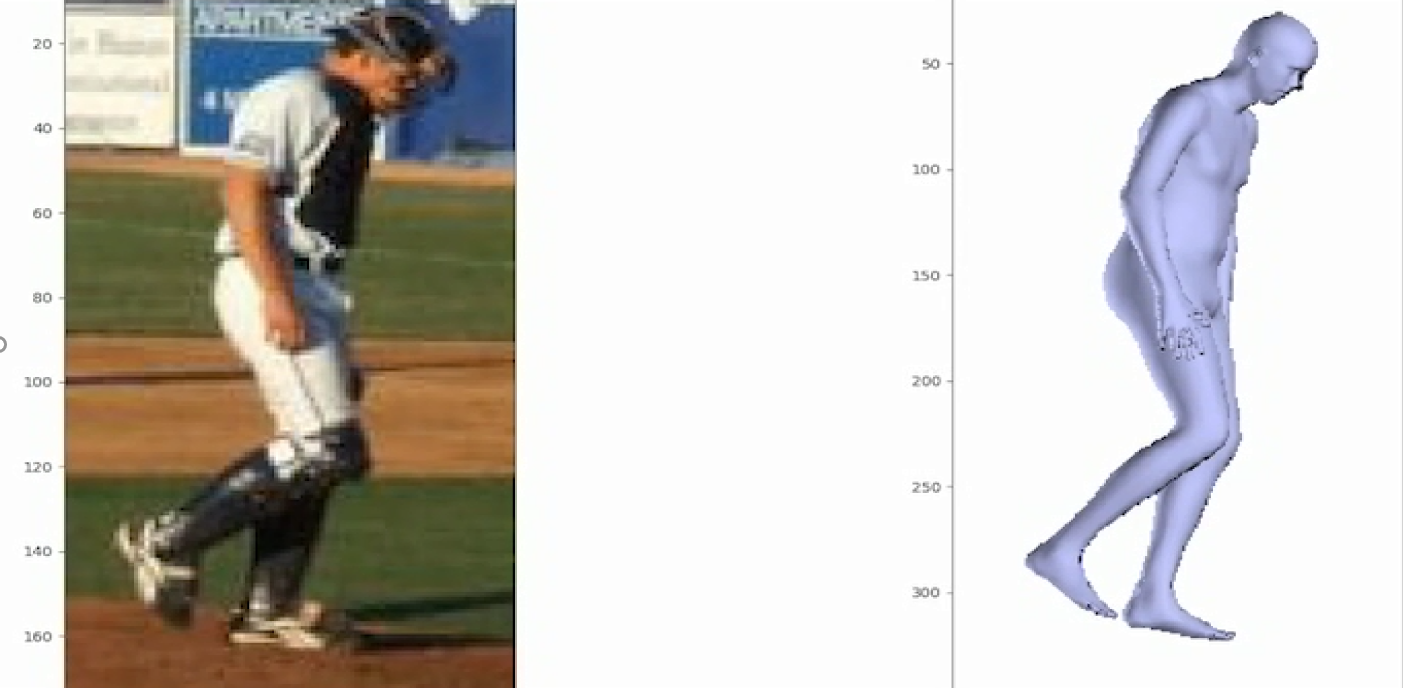
\includegraphics[width=0.95\linewidth]{fitting_smpl}}
        \caption{SMPLify: Fitting the SMPL model to the Leeds Sports Dataset.}
        \label{fig:smplify}
    \end{figure}
        
    \subsubsection{Direct regression}
    The most recent, and state-of-the-art approaches employ deep learning techniques to solve the entire optimization problem by directly regressing shape and pose parameters of the template model. An early approach by Tan et al.~\cite{tan17indirect} used deep neural networks to learn an encoding $f: \RR{H}{W} \mapsto (\pose, \shape, \trans, K)$ of input images to SMPL pose and shape, translation and camera parameters. Their method makes use of a \emph{silhouette renderer} $R : (V, T) \mapsto \{0,1\}^{H \times W}$ (learnt using synthetic data) capable of producing a binary silhouette from a predicted SMPL mesh. In this way, $R$ allows the network's SMPL predictions to be supervised to ensure generated silhouettes match ground-truth annotations. 
    Improvements were realised by incoporating an abudance of available human data into the training pipeline. Apart from 3D morphable models (e.g. SMPL~\cite{loper15smpl}), methods use paired 3D motion capture data (e.g. Human3.6M~\cite{ionescu2013human3,IonescuSminchisescu11}, 3DPW~\cite{vonmarcard2018recovering}) to help relate 2D appearance and the underlying 3D structure, unpaired 3D motion capture data (e.g. CMU~\lazycite{CMU}{CMU}) for learning detailed priors over the distribution of human shapes and poses, and large 2D keypoint datasets (e.g. MSCOCO~\lazycite{COCO}{COCO}, LSP~\lazycite{LSP}{LSP}, MPI~\lazycite{MPI}{MPI}) which help promote generalization to `in-the-wild' scenarios. A notable work in this category is Human Mesh Recovery (HMR) of Kanazawa et al.~\cite{kanazawa18end-to-end}, although multiple concurrent works exist\lazycite{https://proceedings.neurips.cc/paper/2017/file/ab452534c5ce28c4fbb0e102d4a4fb2e-Paper.pdf}{Hsiao-Yu Fish Tung}, \lazycite{https://www.seas.upenn.edu/~pavlakos/projects/humanshape/}{pavlakos}, \lazycite{http://virtualhumans.mpi-inf.mpg.de/papers/omran2018NBF/omran2018NBF.pdf}{neural body fitting} and \lazycite{DenseRaC}{DenseRaC}. \Cref{chap:3dmulti} of this thesis will explore a method for modelling uncertainty in 3D reconstruction, by exploring extensions to the aforementioned architectures.

    % Show the basic structure of these networks in a picture
    
    BodyNet \lazycite{https://www.di.ens.fr/willow/research/bodynet/}{bodynet} follow a similar pipeline with the inclusion of a texture prediction module supervised by 2D body part segementations \lazycite{body part dataset}{dataset}. Silhouette data has also been shown to assist in accurate reconstruction of clothes, hair and other appearance detail~\cite{alldieck2019learning} \lazycite{https://arxiv.org/pdf/1901.00049.pdf}{SiCloPe} \lazycite{https://arxiv.org/abs/2004.04572}{ARCH}. Methods typically represent 3D clothes as `freeform' vertex deformations; in other words, deformations beyond the standard SMPL blend shapes which represent unclothed bodies. This presents significantly more degrees of freedom in the optimization, which must be controlled; either by large training datasets with limited variation or mesh-based deformation priors such as ARAP. 

    While the dominant paradigm in human reconstruction is now end-to-end deep learning methods, SPIN~\cite{kolotouros19learning} show impressive improvement by incorporating an energy minimization process within their training loop to further minimize a 2D reprojection loss subject to fixed pose \& shape priors. This idea inspired the work presented in \Cref{chap:wldo} of this thesis, in which a 3D dog shape prior is learnt during the training loop via expectation maximization.

    % https://openaccess.thecvf.com/content_ICCV_2019/papers/Xu_DenseRaC_Joint_3D_Pose_and_Shape_Estimation_by_Dense_Render-and-Compare_ICCV_2019_paper.pdf
    
    There have also been a few recent works that reconstruct 3D humans without an explicit template prior. The general idea is to interpret a neural network as an implicit representation of the 3D surface. In particular, the network $f$ is trained to map sampled 3D locations $(x,y,z) \in \R{3}$ to an occupancy value $\{0,1\}$ (and optionally a texture value $(r,g,b) \in \R{3}$). This results in a memory efficient representation of the 3D surface as the space used to embed the surface does not need to be explicitly stored. Saito et al.~\cite{pifuSHNMKL19,saito2020pifuhd} present an example of such an architecture. Their network maps 3D locations with ResNet~\lazycite{Resnet}{Resnet} features sampled at coordinates projected with a known weak-perpective camera to occupancy and texture values. Li et al.\lazycite{https://project-splinter.github.io/monoport/}{MonoPort} later sped up reconstruction and rendering to allow real-time inference. Neural Radiance Fields (NeRF) capture high resolution details of static scenes by mapping 3D coordinates $(x,y,z)$ and viewing directions $(\theta, \phi)$ to volume density and view-dependent emitted radiances. The work was adapted to articulated structures~\lazycite{ANerf}{ANerf} by learning new skin for the SMPL model, using SPIN~\cite{kolotouros19learning} as a basic 3D skeleton predictor. A current downside of these techniques is the need to train a separate model per scene/subject and the slow inference time. However, these works do demonstrate high quality results and are a worthy direction for future research.

    % Show the basic structure of these networks in a picture

\subsection{Model-based animals}

    Having discussed reconstruction methods for other articulated subjects, this section will move on work related to the main topic of this thesis: 3D reconstruction of animal subjects. As summarized above, there are multiple challenges associated with animals which are not present with humans. Firstly, the general class of animal subjects is significantly more diverse in appearance and structure than the human category. This holds (although to a lesser extent) with various important animal subcategorizations, such as the class of medium-to-large quadrupeds, dog breeds, or birds. This diversity leads to challenges when designing 3D morphable models, since extreme deformations must allowed while penalizing even subtle adapations deemed unnatural. Also of concern are the significant variations in animal motion patterns (causing complex self-occlusion), body textures including fur (which vary even within breeds) and difficult environmental conditions. An interesting advantageous aspect to reconstructing animals is that they are less frequently clothed; a common nusiance factor for human reconstruction. These factors combined with practical challenges associated with capturing and annotating images has also led to a lack of open-source datasets which depict animal subjects. Of particular concern to this thesis is the lack of 3D training data captured from real animal subjects (typically using motion capture or static scans). Equivalent resources made available for humans have been used as a basis for building 3D morphable models (e.g. SMPL~\cite{loper15smpl}, FAUST~\lazycite{FAUST}{FAUST}), for learning priors over human shape and pose~\lazycite{learning priors}{learning priors}, and to provide per-image 3D supervisation when training deep neural networks~\cite{kanazawa18end-to-end}. Thankfully, online animal imagery which could serve as the basis for future datasets is plentiful, as are datasets with 2D silhouette data~\cite{lin2014microsoft,everingham2010pascal,DAVIS2017-2nd}. A formal comparison is given in \Cref{tab:animal-dsets}.  While animals are often featured in computer vision literature, there are still relatively few works that focus on accurate 3D animal reconstruction. However, the creative approaches used in these methods makes a formal review worthwhile. A summary of recent approaches is tabulated in \Cref{tab:literature}.
    
    % Please add the following required packages to your document preamble:
% \usepackage{booktabs}
\begin{table}[]
    \begin{tabular}{@{}lllll@{}}
    \toprule
    Dataset & Modality & Annotation & Subject & Num. Examples \\ 
    \midrule
    MSCOCO~\cite{lin2014microsoft} & Image (RGB) & S2, BB2 & DCaHoZSECoBG & 23,467 \\
    PascalVOC~\cite{everingham2010pascal} & Image (RGB) & S2, BB2 & xxx & xxx \\
    DAVIS~\cite{DAVIS2017-2nd} & Video (RGB) & S2 & xxx & xxx \\
    StanfordDogs & Image (RGB) & BB2 & D (120 breeds) & 20,580 \\
    \textbf{StanfordExtra} & Image (RGB) & J2, S2 & D (120 breeds) & 12,000 \\
    \textbf{BADJA} & Video (RGB) & J2, S2 & xxx & xxx \\
    AnimalPose & Image (RGB) & J2 & xxx & xxx \\
    SMAL & N/A & MM3 & DCaHoZCoTLHi & 47 \\
    \bottomrule
    \end{tabular}
    \caption{Dataset summary: analysis of available datasets. 
        Bold rows are datasets introduced in this thesis.
        S2: 2D Silhouettes, BB2: 2D bounding boxes, J2: 2D Joints, 
        MM3: 3D Morphable Model. P3: 3D Priors. M3: 3D Model.
        D: dog, Ca: cat, Ho: horse, Z: zebra, S: sheep, 
        E: elephant, Co: cow, B: bear, G: giraffe,
        T: tiger, L: lion: Ch: cheetah, Hi: hippo}
    \label{tab:animal-dsets}
\end{table}

% lin2014microsoft,everingham2010pascal,DAVIS2017-2nd

    

\newcommand{\awfhang}[1]{
    \begin{minipage}[t]{\textwidth}% Top-hanging minipage, will align on
                                   % bottom of first line
    \begin{tabbing} % tabbing so that minipage shrinks to fit
    \\[-\baselineskip] % Make first line zero-height
    #1 % Include user's text
    \end{tabbing}
    \end{minipage}} % can't allow } onto next line, as {WIDEBOX}~x will not tie.
    
    \newcolumntype{L}[1]{>{\RaggedRight\hspace{0pt}}p{#1}}
    \newcolumntype{R}[1]{>{\RaggedLeft\hspace{0pt}}p{#1}}
    
    \begin{table}[t!]
    {\sffamily
    \scriptsize
    \def\hd#1{\awfhang{#1}}
    \begin{tabular}{@{}L{20mm}%Paper
    |L{12mm}%Class
    L{15mm}%Train
    |L{15mm}%Template
    L{17mm}%Video
    L{17mm}%Test
    |L{9mm}%Model
    L{5mm}%Size
    @{}}
    \hd{Paper}%
    &\hd{Animal\\Class}%
    &\hd{Training\\requirements}%
    &\hd{Template\\Model}%
    &\hd{Video\\required}%
    &\hd{Test Time\\Annotation}%
    &\hd{Model\\Fitting}%
    &\hd{Test\\Size}%
    \\\hline
    %%%%%%%%%%%%%%%%%%%%%%
    This paper
    & Dogs  % 2D Joints, Silhouettes, 3D Template, 3D Priors
    & J2, S2, T3, P3
    & SMAL
    & No & None & No & 1703
    \\\hline
    %%%%%%%%%%%%%%%%%%%%%%
    3D-Safari~\cite{Zuffi19Safari}        
    & Zebras, horses
    % 3D models (albeit synthetic), 2D Joints,  Silhouettes,  3D Priors
    & M3 (albeit synthetic), J2, S2, P3
    & SMAL
    & 3-7 frames / animal & None & Yes & 200
    \\\hline
    %%%%%%%%%%%%%%%%%%%%%%
    Lions, Tigers and Bears (SMALR)~\cite{zuffi_lions} 
    & MLQ
    & Not trained
    & SMAL
    & 3-7 frames / animal & J2, S2 & Yes & 14
    \\\hline
    %%%%%%%%%%%%%%%%%%%%%%
    3D Menagerie (SMAL)~\cite{zuffi2017menagerie}                
    & MLQ 
    & Not trained
    & SMAL
    & No & J2, S2 & Yes & 48 
    \\\hline
    %%%%%%%%%%%%%%%%%%%%%%
    Creatures Great and SMAL~\cite{biggs2018creatures}
    & MLQ
    & Not trained
    & SMAL
    & Yes & S2 (for best results shown) & Yes & 9             \\\hline 
    %%%%%%%%%%%%%%%%%%%%%%
    Category Specific Mesh Reconstructions~\cite{kanazawa2018birds}
    & Birds
    & J2, S2
    & Bird convex hull
    & No & None & No & 2850          
    \\\hline
    %%%%%%%%%%%%%%%%%%%%%%
    What Shape are Dolphins~\cite{cashman2013shape}
    & Dolphins, Pigeons 
    & Not trained
    & Dolphin Template
    & 25 frames / category & J2, S2 & Yes & 25
    \\\hline
    %%%%%%%%%%%%%%%%%%%%%%
    Animated 3D Creatures~\cite{reinert2016animatedsketching}
    & MLQ
    & Not trained
    & Generalized Cylinders
    & Yes & J2, S2 & Yes & 15
    \\\hline
    \end{tabular}
    }
    \caption{Literature summary: Our paper extends large-scale ``in-the-wild'' reconstruction to the difficult class of diverse breeds of dogs. 
    MLQ: Medium-to-large quadrupeds. J2: 2D Joints. S2: 2D Silhouettes. T3: 3D Template. P3: 3D Priors. M3: 3D Model.}
    \label{tab:literature}
    % \vspace{-8mm}
    \end{table}
    
    

    % Table~\ref{tab:literature} summarizes previous work on animal reconstruction.
    % It is interesting to note that while several papers demonstrate reconstruction across species, which {\em prima facie} is a richer class than just dogs, the test-time requirements (e.g. manually-clicked keypoints/silhouette segmentations, input image quality etc.) are considerably higher for those systems.
    % Thus we claim that the achievement of reconstructing a full range of dog breeds, 
    % with variable fur length, varying shape and pose of ears, and with considerable occlusion, is a significant contribution.

    % \subsubsection{Animals intro}

    % Cashman and Fitzgibbon~\cite{cashman2013shape} obtained one of the first 3D morphable animal models, but their work was limited to small classes of objects (e.g. dolphins, pigeons), and did not incorporate a skeleton.  Their work also showed the use of the 2D silhouette for fitting, which is key to our method. 
    % Reinert {\em et al.} \cite{reinert2016animated} meanwhile construct 3D meshes by fitting generalized cylinders to hand-drawn skeletons.
    % Combined skeletal and morphable models were used by Khamis {\em et al.}~\cite{hand-shape} for modelling the human hand, and Loper {\em et al.}~\cite{loper15smpl} in the SMPL model which has been extensively used for human tracking. 

    % The SMPL model was extended to animals by Zuffi {\em et al.}~\cite{zuffi2017menagerie}, where the lack of motion capture data for animal subjects is cleverly overcome by building the model from $41$ 3D scans of toy figurines from five quadruped families in arbitrary poses. Their paper demonstrates single-frame fits of their model to real-world animal data, showing that despite the model being built from ``artists' impressions'' it remains an accurate model of real animals. This is borne out further by our work.  Their paper did however depend on per-frame human annotated keypoint labels, which would be costly and challenging to obtain for large video sequences. This work was recently extended~\cite{zuffi_lions} with a refinement step that optimizes over model vertex positions. This can be considered independent to the initial SMAL model fit and would be trivial to add to our method.

    \subsubsection{Learning animal shape from 2D image collections}
    % Early work in reconstructing animals includes Chen et al.~\lazycite{chensharks}{chensharks} who learn a simple shape space by registering 11 3D shark models. 
    
    Early work in animals focuses on learning 3D animal shape spaces by registering an input 3D model to image collections. Examples include Chen et al.\lazycite{chensharks}{chensharks} who learn a shark model and Cashman et al.~\cite{cashman2013shape} who recover a parameterized, morphable 3D model from unrelated 2D images depicting examples of the target class. Their method requires user-supplied 2D object outlines and point constraints for each image, and a single rigid mesh for the entire object class. The authors demonstrate recovering an 8-parameter morphable dolphin model from 32 images sourced from the Internet. To reduce required user activity, it is reasonable to assume that given sufficient labelled training data, it would be simple to manipulate a convolutional network architecture able to perform foreground / background segmentation and identify key points (say, joints) for the desired object class. The system achieves impressive results when optimizing over both pose and shape parameters across a range of object classes, but suffers from an overly smooth shape representation which causes trouble for strongly articulated classes such as polar bears. Related is the work of Ntouskos et al.\lazycite{ntouskos}{ntouskos} who use an optimization scheme to combine geometric primitives fit to segmented animal parts.

    \begin{figure}[t] % Example image
        \center{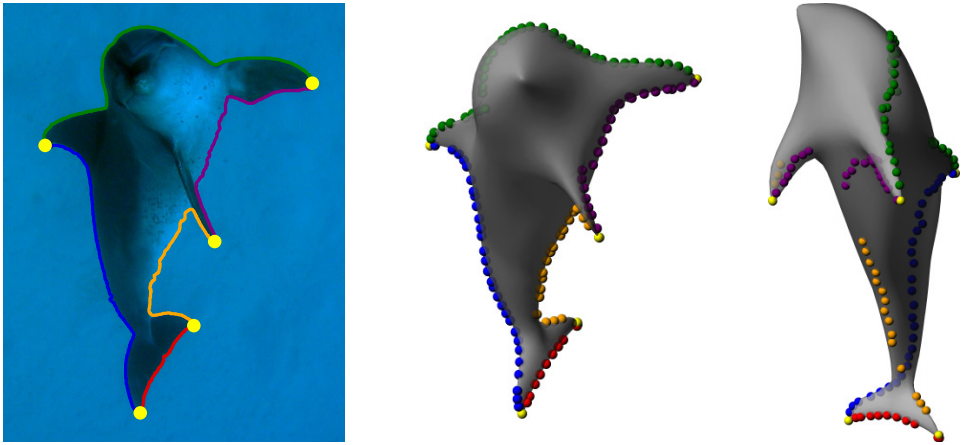
\includegraphics[width=0.7\linewidth]{dolphins}}
        \caption{8-parameter dolphin model with annotated contour (left) and contour generators (middle and right).}
        \label{fig:cashman_fitzgibbon}
    \end{figure}

    
    \subsubsection{Reconstructing animals with unknown skeleton}

    The approach was later extended to articulated classes in work by Stebbing et al.~\cite{arap_stebbing}, who optimize a 3D template model to animal video sequences. In this work, rather than defining an internal skeleton, the template model is rigged with virtual markers, which assign each mesh vertex $v_i$ to one of $M$ groups that share a set of basis rotations $B_{m}$. User interaction is again reuqired to segement the animal from the background and to provide mesh-to-image keypoint correspondences.

    \begin{figure}[t]
        \centering
        \begin{subfigure}{0.5\textwidth}
        \centering
            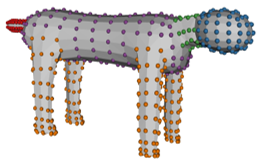
\includegraphics[height=0.5\linewidth]{arapsfm/arap_annotated_template}
            \caption{Template mesh with joint movement constraints.}
        \end{subfigure}%
        \begin{subfigure}{0.5\textwidth}
        \centering
            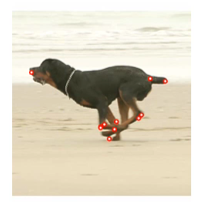
\includegraphics[height=0.5\linewidth]{arapsfm/arap_point_tracks}
            \caption{Example of user supplied point tracks.}
        \end{subfigure}%
        \caption{User input required for the deformable mesh animation algorithm, reprinted from~\cite{arap_stebbing}.}
        \label{fig:arap_user}
    \end{figure} 

    Through reasonably accurate pose fitting and by allowing some pose-invariant shape deformation, this work produces smooth meshes which match the input video. Moreover, experimentation demonstrates that ARAP is a useful prior for reconstructing articulated, non-rigid motion in instances that an internal skeleton is a priori unknown. However, the shape attributes for the reconstructed model are not particularly accurate, which results in frequent errors appearing at internal occluding contours. In addition, the large non-convex optimization algorithm is an expensive operation, taking around 1 minute per video frame on a standard Linux workstation. Results are shown on 11 sequences.

    Results showing this work fitting a crude dog template mesh to a sample video obtained from YouTube are shown previously in Figure \ref{fig:intro_arap_output}. Figure \ref{fig:arap_output} shows another example, which operates on a template impala mesh. Similar is the technique of Favreau et al.~\lazycite{favreau}{favreau}, who fitting geometric primitives to a 2D video sequence with manually sketched body part labels. % TODO

    \begin{figure}[t]
        \center{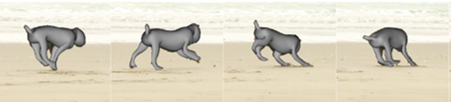
\includegraphics[width=0.95\linewidth]{arapsfm/arapsfm_output.png}}
        \caption{Example of an dog template being fit to input video sequence, reprinted from~\cite{arap_stebbing}}
        \label{fig:arap_output}
    \end{figure}

    \subsubsection{Fitting a morphable animal mesh to images}
    % Draw out the silhouette term as important here
    % Talk about subsequent SMALR + SMALST in the same section
    Unfortunately, none of the techniques above are suitable for reconstructing an animal category with significant shape diversity.     Zuffi et al.~\cite{zuffi2017menagerie} made a significant contribution by releasing SMAL, a deformable 3D quadruped model (analagous to SMPL~\cite{loper15smpl} for human reconstruction) build from $41$ scans of artist-designed toy figurines. The authors also released shape and pose priors generated from artist data. The authors also discuss a small modification to the SMPLify~\lazycite{smplify}{smplify} approach in order to fit the SMAL model to RGB animal input images. However, an example result showing the result of the optimizer fitting the SMAL mesh to an RGB image of a fox can be seen in Figure \ref{fig:smalify}. The whole optimization process takes around 1 minute per frame. 

    \begin{figure}[t] % Example image
        \center{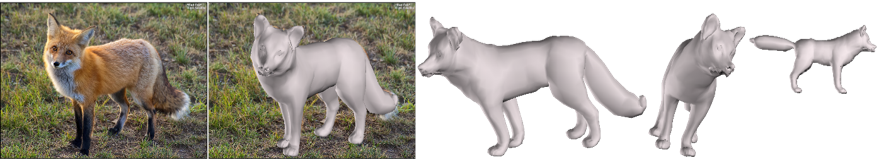
\includegraphics[width=0.95\linewidth]{fitting_smal}}
        \caption{Fitting SMAL to a hand segmented animal, reprinted from~\cite{zuffi2017menagerie}.}
        \label{fig:smalify}
    \end{figure}

    The terms of the optimization largely mirror the work of SMALify, although the interpenetration term is ommited and joints are provided manually rather than by a CNN. Importantly, the optimization incoporates an additional \emph{silhouette} term which aligns the 3D model shape to a binary silhouette image extracted by a user. \Cref{chap:cgas} of this thesis shows silhouette terms are of particular importance when reconstructing accurate animal shape. The following definition describes the process for differentiably rendering a 3D model to form a silhouette image which can then be compared to the provided 2D silhouette:

    \begin{definition}[Differentiable Rendering]
        The process of generating a 2D image from a 3D polygon mesh is known as rendering and can be achieved through a process known as raytracing. Raytracing is a rendering technique able to generate photorealistic 2D images from the scene. It can be considered the opposite process by which the human eye perceives the world, as this method involves lines being cast outwards, beginning at a point known as the \emph{camera origin}. Figure \ref{fig:raycasting} shows a typical set up, in which rays are cast from the camera origin through each pixel on the image plane. The colour for the pixel is obtained by following the ray through the scene until a light source or non-reflective surface is reached, taking into account any reflections or non-opaque scene items. Due to the considerable comptuation required, the operation is often parallelized and assigned to the GPU. However, the technique is typically considered unsuitable for real-time rendering of complex scenes (due to complex ray paths) or when high resolution images (many rays required) are needed. However, for this work, scenes are typically made up of a single non-reflective, solid mesh surface and contain no complex elements (e.g.\ shadows, non-constant lighting.

        \begin{figure}[H] % Example image
            \center{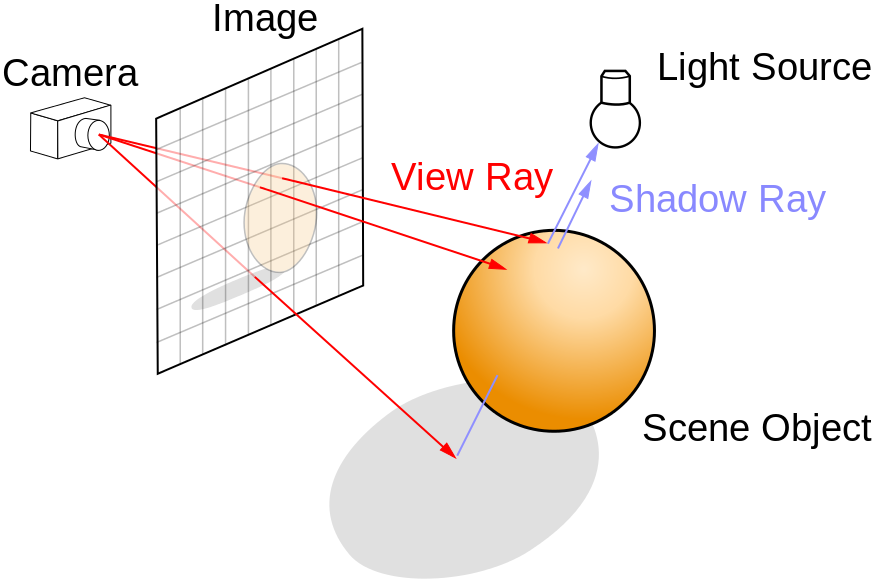
\includegraphics[width=0.5\linewidth]{ray_trace}}
            \caption{Diagram showing raycast rendering.~\cite{rendering}.}
            \label{fig:raycasting}
        \end{figure}

        It is also worth noting that the standard method for raycasting is not differentiable, causing problems for differentiable optimizers (including neural networks). However, alternative rendering methods~\cite{loper2014opendr} are available for these purposes.
    \end{definition}

    The SMAL authors~\cite{zuffi2017menagerie} demonstrate their system by fitting their deformable 3D model to quadruped species. Subsequent work includes SMALR~\cite{zuffi_lions}, who fit to multiple images of an animal and incoporate similar freeform deformation term used to model clothing in 3D human pipelines. They show their technique, which takes advantage of multi-view constraints afforded by fitting to video sequences, allows high-quality reconstructions of more exotic animal categories with details not covered in the original SMAL 3D model training set. 
    
    A common property of techniques discussed so far is the reliance on manual annotations (commonly 2D silhouettes and keypoint correspondences) at test time. 3D-Safari~\cite{Zuffi19Safari} overcome this by training a deep network on synthetic data (generated by applying SMALR~\cite{zuffi_lions} on a large input dataset) to recover detailed zebra shapes in the wild. \Cref{chap:cgas} of this thesis demonstrates a technique which overcomes the need for a large input dataset of joint annotations by training on synthetic data generated from the graphics model alone. 
    
    A further drawback of the approaches is their reliance on a test-time energy-based optimization procedure, which is susceptible to failure with poor quality keypoint/silhouette predictions and increases the computational burden. \Cref{chap:wldo} of this method presents an automatic reconstruction method that overcomes the need for additional energy-based refinement, and is trained purely from single in-the-wild images. 
    
    Tangential to these approaches is the work of Kulkarni et al.\lazycite{Canonical Surface Mapping}{Canonical Surface Mapping} who reconstruct pose (although not shape) parameters for an rigged mesh using a deep network, learning from geometry cycle consistency terms rather than annotated keypoints. However, the shape is fixed to the input mesh and pose is also often confused, particularly determining the difference between the legs. The results appear of significantly poorer quality than the results in \Cref{chap:cgas} and \Cref{chap:wldo} of this thesis. Also of consideration is the end-to-end network of Kanazawa et al.~\cite{kanazawa2018birds} and subsequent paper which overcomes the need for keypoints by capturing uncertainty in camera viewpoints. In addition, their network does not require an input 3D morphable model, although they do initialize a sphere model to a mean bird. In addition, the bird category exhibits more limited articulation than our dog category. 
    
    
    % TODO:
    %Finally, there are techniques which do not produce a mesh~\cite{Agudo_2018_CVPR,novotny19c3dpo} or rely heavily on input 2D keypoints or video at test-time~\cite{vicente_3dv,Probst2018_ECCVa}.
    % Unsupervised Learning of Probably Symmetric Deformable 3D Objects from Images in the Wild
    % Canonical Surface Mapping via Geometric Cycle Consistency https://arxiv.org/abs/1907.10043



% \subsubsection{Literature review tables}

% The closest work in terms of scale is the category-specific mesh reconstruction of Kanazawa et al.~\cite{kanazawa2018birds}, where 2850 images of birds were reconstructed.  However doing so for the complex pose and shape variations of dogs required the advances described in this paper.



